\section{Motions}
\begin{frame}
	\frametitle{Lecture III Outline}
	\begin{tcolorbox}[coltitle=yellow!50!black,colframe=magenta!25,split=.2,title=Lecture III Outline]
		Rigid Body Transformations and Screws Theory.
		\tcblower
		Rigid body motions: Properties; Direction cosines; Rotation compositions; Rotation Parameterizations.
		\vspace{.2cm}
		\newline
		Rodrigues' formula; the matrix exponential, $SO(3), SO(n), \mathbb{SE}(3)$ group properties.
		\vspace{.2cm}
		\newline
		Transformations: Translations and rotations in $\mathbb{R}^3$, planar rotations, $SO(3), SE(3)$ motions;  homogeneous transformations; Euler and Fick angles.  
	\end{tcolorbox}
\end{frame}


\begin{frame}
	\frametitle{Rigid Body Motions}
	%
	\begin{block}{Rigid Body Motion -- Intro}
		A mapping $g:  \mathbb{R}^3  \rightarrow \mathbb{R}^3$ is a \textcolor{red}{rigid body motion} if 
		\begin{align}
			\|g({x}) - g({y})\| &= \|{x} - {y}\| \text{ for all }  {x}, {y} \in \mathbb{R}^3;  \\
			g({x} \times {y}) &= g(x) \times g({y})\text{ for all }  {x}, {y} \in \mathbb{R}^3; 
		\end{align}
	\end{block}	
	%
	\begin{block}{Rigid Body Motion Preserves Inner Products}
		For two vectors $\bm{a}$ and $\bm{b}$,  $\langle \bm{a},  \bm{b}\rangle =  g(\bm{a}) \times  g(\bm{b})$.
	\end{block}
\end{frame}



\subsection{Movement in $\mathbb{R}^3$}
\begin{frame}
	\frametitle{Rigid Body Transformations}
	%
	\begin{block}{Translation of Point $\bm{q}$ between Two Frames}
		For a reference frame, $o_0 x_0 y_0$ and a moving coordinate frame, $o_1 x_1 y_1$, the translation of $\bm{q}$ is given as below:
	\end{block}
	\begin{columns}[]
		\begin{column}{.5\linewidth}
			\centering
			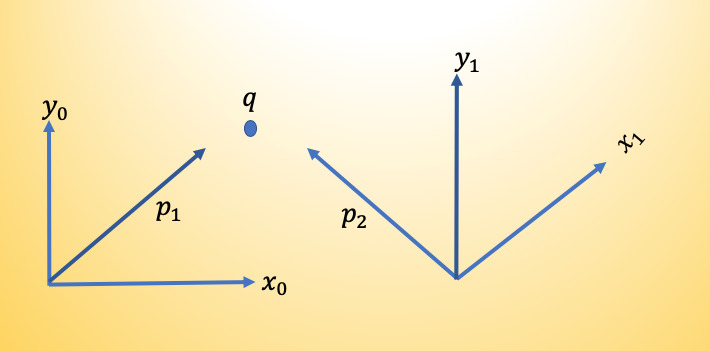
\includegraphics[width=\textwidth]{../Notes/figures/trans_coords.jpg}
		\end{column}
		\begin{column}{.5\linewidth}
			\begin{align}
				q^0 = \left( \begin{array}{c}
					q^0_x \\ q_y^0
				\end{array}
				\right), \quad
				%
				q^1 = \left( \begin{array}{c}
					q^1_x \\ q_y^1
				\end{array}
				\right) \nonumber
			\end{align}
		\end{column}
	\end{columns}
	%
	\begin{block}{Translation of Origin between Two Frames}
		\begin{align}
			o^0_1 = \left( \begin{array}{c}
				o^0_x \\ o^0_y
			\end{array}
			\right), \quad
			%
			o^1_0 = \left( \begin{array}{c}
				o^1_x \\ o^1_y
			\end{array}
			\right).
		\end{align}
	\end{block}
\end{frame}

\begin{frame}
	\frametitle{Rigid Body Transformations}
	%
	\begin{block}{Applications to Screws}
		Applies to Chasles' displacement theorem and Poinsot's force and couple transformations too.
	\end{block}
	%
	\begin{block}{Screw Transformations}
		\begin{align}
			\bm{t}^0_1 &= \left( \begin{array}{c}
				t^0_x \\  t^0_y %\\  t^0_z
			\end{array}
			\right),
			%
			\quad \bm{t}^1_1 = R(-\theta) q^0 \\
			%
		    \bm{t}^0_2 &= R(\theta) q^0, \quad \bm{t}^1_2 = \left( \begin{array}{c}
				t^1_x \\  t^1_y %\\  t^1_y
			\end{array}
			\right)
		\end{align}
		%
		where $\theta$ is the angle coordinate frame $o_1 x_1 y_1$ makes w.r.t $o_0 x_0 y_0$.
	\end{block}
\end{frame}

\begin{frame}
	\frametitle{Rotations in $\bb{R}^3$}
	%
	\begin{block}{Rotations in $\bb{R}^3$}
		Conventions: Bodies' \textcolor{blue}{orientations} are \textcolor{magenta}{measured along a corkscrew direction}, specified by a \textcolor{cyan}{local coordinate frame}. Thus, \textcolor{magenta}{relative orientation} is measured from the \textcolor{cyan}{local coordinate frame} to an \textcolor{magenta}{inertial coordinate frame}.
	\end{block}
	%
\end{frame}

\begin{frame}
	\frametitle{Direction Cosines}
	%
	\begin{columns}[]
		\begin{column}{.6\linewidth}
			\centering
			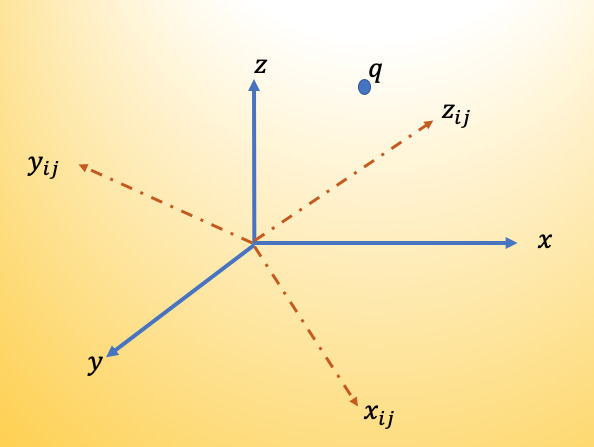
\includegraphics[width=\textwidth]{../Notes/figures/rotation_illus.jpg}
		\end{column}
		\begin{column}{.4\linewidth}
			\begin{block}{Conventions}
			 $I$: \textcolor{magenta}{Inertial frame}; $J$: \textcolor{cyan}{Body frame}.
				%
			$\bm{q}: (\bm{x}_{ij}, \bm{y}_{ij},\bm{z}_{ij}) \in \bb{R}^3$: coordinates of the \textcolor{purple}{principal axes} of $J$ relative to $I$.
			\end{block}
		\end{column}
	\end{columns}
\end{frame}


\begin{frame}
	\frametitle{Rotation Matrix from Direction Cosines}
	\begin{block}{Rotation as Composition of Projections Between Frames}
		\begin{align}
			R_{ij} = \begin{bmatrix}
				\bm{x}_{ij} \quad  \bm{y}_{ij} \quad \bm{z}_{ij}
			\end{bmatrix} = \begin{bmatrix}
				r_{11} &  r_{12} & r_{13} \\
				r_{21} & r_{22} &  r_{23} \\
				r_{31} & r_{32} &  r_{33}
			\end{bmatrix}.
			\label{eq:rotation_compoz}
		\end{align}
	\end{block}
	
	\begin{block}{Rotation Matrix as Unit Axes' Dot Products}
		\begin{align}
			R_{ij} = \begin{bmatrix}
				\bm{x}_j \cdot \bm{x}_i & \bm{y}_j \cdot \bm{x}_i & \bm{z}_j \cdot \bm{x}_i \\
				%
				\bm{x}_j \cdot \bm{y}_i & \bm{y}_j \cdot \bm{y}_i & \bm{z}_j \cdot \bm{y}_i \\
				%
				\bm{x}_j \cdot \bm{z}_i & \bm{y}_j \cdot \bm{z}_i & \bm{z}_j \cdot \bm{z}_i 
			\end{bmatrix}.
			\label{eq:direction_cosines}
		\end{align}
	\end{block}
\end{frame}

\begin{frame}
	\frametitle{Rotation Matrix from Direction Cosines}
	\begin{block}{Rotation Matrices are Direction Cosines!}
		$\bm{x}_j \cdot \bm{x}_i = \cos(\measuredangle\left(\bm{x}_j, \bm{x}_i\right)), \quad 	\bm{y}_j \cdot \bm{x}_i = \cos(\measuredangle\left(\bm{y}_j, \bm{x}_i\right)), \cdots$
		
		$\cdots, \bm{y}_j \cdot \bm{z}_i = \cos(\measuredangle\left(\bm{y}_j, \bm{z}_i\right)), \quad 	\bm{z}_j \cdot \bm{z}_i = \cos(\measuredangle\left(\bm{z}_j, \bm{z}_i\right)).$
	\end{block}
	
	\begin{block}{Properties of Rotation Matrices}
		Rows of $R_{ij}$ are the \textcolor{magenta}{unit vector} coordinates of $I$  in the frame $J$ so that 
		%
		\begin{align}
			R_{ij} =  R_{ji}^{-1} = R_{ji}^T.
		\end{align}
		%
		That is, the \textcolor{blue}{inverse of the rotation matrix is equal to its transpose}. 
	\end{block}
\end{frame}

\subsection{Special Orthogonal Properties}
\begin{frame}
	\frametitle{Special Orthogonal 3, SO(3)}
	\begin{block}{Orthogonal properties!}
			Observe: $\text{det }  \bm{R} = \bm{r}_1^T \cdot \left(\bm{r}_2 \times \bm{r}_3\right)$. In \textcolor{cyan}{corkscrew notation}, $\text{det }  \bm{R} = +1$ i.e. $\bm{r}_2 \times \bm{r}_3 = \bm{r}_1$ so that $\text{det }  \bm{R} = \bm{r}_1^T \cdot \bm{r}_1 = +1$. A matrix that satisfies the above property is said to \textcolor{light-blue}{possess a special orthogonal 3, denoted SO(3),  property}.
	\end{block}
	
	\begin{block}{SO(n) Property}
		Special orthogonal means $\text{det } \bm{R} = + 1$. The set of all SO matrices in $\bb{R}^{n\times n}$ is 
		%
		\begin{align}
			\text{SO(n)} = \{\bm{R}\in \bb{R}^{n\times n}: \bm{R}\cdot \bm{R}^T = \bm{I}, \text{det }\bm{R} = + 1\}.
		\end{align}
	\end{block}
\end{frame}

\begin{frame}
	\frametitle{Rotations on Vectors}
	\begin{columns}[]
		\begin{column}{.85\linewidth}
			\begin{block}{Rotating a Vector}
				Suppose that a point $p_j$ is on a frame $J$, then the vector that connects a point $q_j$ in the frame $J$ to $p_j$ is $v_j = q_j - p_j$. Now, the rotation matrix's action on $v_j$ is
				%
				\begin{align}
					\bm{R}_{ij}(v_j) := \bm{R}_{ij} q_j - \bm{R}_{ij} p_j = q_i - p_i = v_i.
				\end{align}
			\end{block}
		\end{column}
	\end{columns}
\end{frame}


\begin{frame}
	\frametitle{Planar Rotations}
	\begin{columns}[]
		\begin{column}{.5\linewidth}
			\begin{block}{Planar Rotations}
				Let the angle of rotation between the two coordinate frames be $\theta$. Then,
			\begin{align}
				R_1^0 = \left(\begin{array}{cc}
					x_1^0 \,\,| & y_1^0
				\end{array}\right)
			\end{align}
			\end{block}
		\end{column}
		\begin{column}{.5\linewidth}
			\centering
			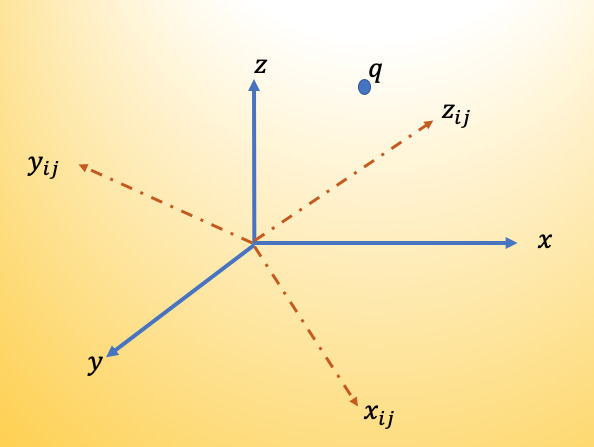
\includegraphics[width=\textwidth]{../Notes/figures/rotation_illus.jpg}
		\end{column}
	\end{columns}
	
	\begin{columns}[]
		\begin{column}{.5\linewidth}
			\begin{block}{Planar Rotations}
				It follows that
				\begin{align}
					R = \left(\begin{array}{cc}
						\cos \alpha & -\sin \alpha \\ \sin \alpha &  \cos \alpha
					\end{array}\right)
				\end{align}
			\end{block}
		\end{column}
		\begin{column}{.5\linewidth}
			\centering
			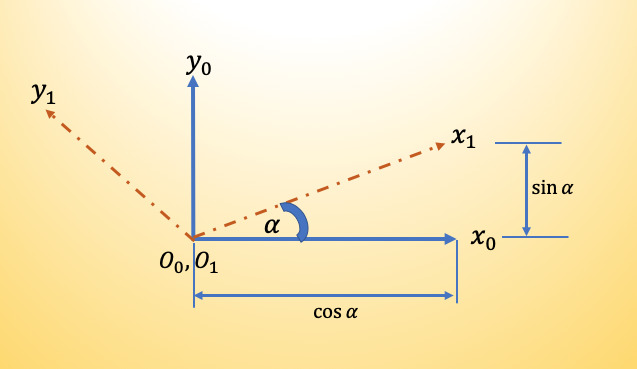
\includegraphics[width=\textwidth]{../Notes/figures/planar_rot.jpg}
		\end{column}
	\end{columns}
\end{frame}


\begin{frame}
	\frametitle{Planar Rotations}
			\begin{block}{Planar Rotations via Direction Cosines}
				\begin{align}
					R_1^0 &= \begin{bmatrix}
						\bm{x}_0 \cdot \bm{x}_1 & \bm{y}_1 \cdot \bm{x}_0 \\
						%
						\bm{x}_0 \cdot \bm{y}_1 & \bm{y}_1 \cdot \bm{y}_0
					\end{bmatrix} =  \begin{bmatrix}
					cos \alpha &  -cos(\pi/2 - \alpha) \\
					%
					cos(\pi/2 - \alpha) & cos \alpha
				\end{bmatrix} \nonumber \\
			%
		&=  \begin{bmatrix}
		cos \alpha &   - \sin \alpha  \\
		%
		\sin \alpha  & cos \alpha
	\end{bmatrix}.
				\end{align}
			\end{block}
		\footnotesize{Projection of $y_1$ on $x_0$ is negative because of our adopted right-handed frame.}
\end{frame}

%\begin{frame}
%	\frametitle{Composition of Rotations About A Current Axis}
%	\begin{block}{Skew Symmetry Operations}
%		%
%		What happens when the \textcolor{red}{order of multiplication is reversed}?
%	\end{block}
%	
%%	\begin{block}{Skew Symmetry}
%%		%
%%		Turns out \textcolor{light-blue}{going from rotations about a current frame} to a \textcolor{blue}{fixed axis} and \textcolor{brown}{rotations from a fixed axis} to a \textcolor{light-red}{current frame} is equivalent to \textcolor{purple}{skew-symmetric operations on matrices} i.e. 
%%		\begin{align}
%%			\bm{R}_{x, \theta} \bm{R}_{z, \psi}  =  \left(\bm{R}_{z, \psi} \bm{R}_{x, \theta}\right)^\wedge
%%		\end{align}
%%	\end{block}
%\end{frame} 

\begin{frame}
	\frametitle{Axis-Angle Parameterization}
	\begin{block}{Exponential Rotation Coordinates}
		It can be verified that 
		\begin{align}
			e^{ \tilde{\omega} \theta} = \identity + \tilde{\omega} \sin \theta + \tilde{\omega}^2 (1 - \cos \theta),
		\end{align}
		 $ \tilde{\omega} \in so(3) \text{ and }so(n) = \{\tilde{\omega}: \tilde{\omega}\in \reline^n \times \reline^n \mid \tilde{\omega}^T = -\tilde{\omega}^T\}$.
	\end{block}
\end{frame}

\begin{frame}
	\frametitle{Axis-Angle Parameterization}
	\begin{block}{Parameterization from Exponentiation of Axial Rotation}
		It can be verified that 
		\begin{align}
			e^{ \tilde{\omega} \theta} = \begin{bmatrix}
				\omega_x^2 v_\theta + c_\theta  & \omega_x\omega_y v_\theta - \omega_z s_\theta & \omega_x \omega_z v_\theta + \omega_y \, s_\theta \\
				%
				\omega_x \omega_y v_\theta + \omega_z s_\theta  & \omega_y^2 v_\theta+ c_\theta & \omega_y \omega_z v_\theta - \omega_x s_\theta \\
				%
				\omega_x \omega_z v_\theta - \omega_y s_\theta  & \omega_y \omega_z v_\theta + \omega_x s_\theta & \omega_z^2 v_\theta + c_\theta
			\end{bmatrix} \nonumber
		\end{align}
		 where $ v_\theta = 1 - \cos \theta$, $-2\pi n \le \theta \le 2\pi n$.
	\end{block}
		\begin{block}{Angle from Exponentiation of Axial Rotation}
		%
		\begin{align}
			%\text{Trace}(\rot) &= r_{11}  + r_{22}  + r_{33} \implies
			 \theta = \cos^{-1}\dfrac{\text{Trace}(\rot)-1}{2}
			 \label{eq:angle_param}
		\end{align}
	\end{block}
\end{frame}

\begin{frame}
	\frametitle{Axis-Angle Parameterization}
	\begin{block}{Axis from Exponentiation of Axial Rotation}
		Equating the off-diagonal terms, we find that
		%
		\begin{align}
			\omega = \frac{1}{2 \sin \theta} \left(
			\begin{array}{c}
				r_{32} - r_{23} \\
				%
				r_{13} - r_{31} \\
				%
				r_{21} - r_{12}
			\end{array} \right)
			\label{eq:axis_param}
		\end{align}
		%
		 Suppose $\theta \neq 0$, equations \eqref{eq:angle_param} together with \eqref{eq:axis_param} are  the \textcolor{brown}{axis-angle representation}.
	\end{block}
\end{frame}


\begin{frame}
	\frametitle{The Skew Symmetrix Matrix}
	\begin{block}{Skew Symmetric Matrix}
		For a \textcolor{brown}{rigid body whose rotation is locally parameterized} by $\rot$ (with $\rot: \rot \rot^T = \identity$) followed by a translation, $\bm{d}$. Compose this transformation as
		%
		%\begin{align}
		$g = \left(\begin{array}{ccc}
			\rot & \identity \\
			0 & 1
		\end{array}\right) \in \liegroup(3)$.
		%\end{align}
	\end{block}
	
	\begin{block}{Skew Symmetric Matrix}
		%
		There exists a \textcolor{brown}{skew symmetric matrix}, $\tilde{\omega}$, for an axis $\omega = [\omega_x, \omega_y, \omega_z]^T$ about which \textcolor{red}{the rotary and translatory} movement occurs such that
		\begin{align}
			\tilde{\omega} = \left(\begin{array}{ccc}
				0 & -\omega_z & \omega_y \\
				\omega_z & 0 & -\omega_x \\
				-\omega_y & \omega_x & 0 
			\end{array}\right) = - \tilde{\omega}^T
		\end{align}
		%Observe $s_{ij} = -s_{ji}$ for $i\neq j$ and $s_ii=0$
	\end{block}
\end{frame}

\subsection{Composition of Rotations}
\begin{frame}
	\frametitle{Composition of Rotations}
	\begin{block}{Rotations Composition}
		Let the \textcolor{cyan}{relative orientation} of a frame $K$  to a frame $J$ be $\bm{R}_{jk}$, and let frame $J$'s  \textcolor{cyan}{relative orientation} to frame $I$ be $\bm{R}_{ij}$, then the \textcolor{cyan}{relative orientation} of frame $K$  w.r.t $I$ is 
		%
		\begin{align}
			\bm{R}_{ik} = \bm{R}_{ij} \cdot \bm{R}_{jk}.
		\end{align} 
	\end{block}
	
	\begin{block}{Rotations Composition}
		Equivalent to \textcolor{brown}{rotating $J$ relative to frame $I$ according to $\bm{R}_{ij}$}; then \textcolor{magenta}{aligning frame $J$  to $K$}, we \textcolor{light-blue}{rotate $K$ relative to $I$ according to $\bm{R}_{jk}$}. This frame relative to which rotation occurs is termed the \textcolor{light-red}{current frame}. 
	\end{block}
\end{frame}


\begin{frame}
	\frametitle{Composition of Rotations About A Current Axis}
	\begin{block}{Composition of Rotations About A Current Axis}
		%
		\centering
		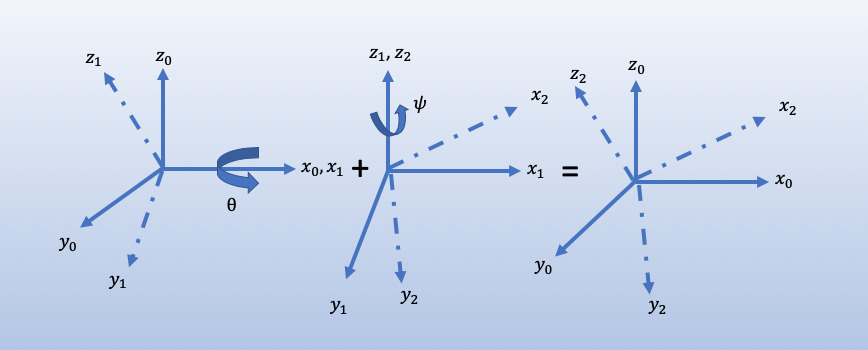
\includegraphics[width=1\textwidth]{../Notes/figures/compoz.jpg}
	\end{block}
\end{frame} 

\begin{frame}
	\frametitle{Composition of Rotations About A Current Axis}
	\begin{block}{Compositions}
		\begin{align}
			\bm{R} &= \bm{R}_{x, \theta} \bm{R}_{z, \psi} 
			%
			= \left(\begin{array}{ccc}
				1 & 0 & 0 \\
				0 & c_\theta & -s_\theta \\
				0 & s_\theta & c_\theta
			\end{array}\right) 
			%
			\cdot
			%
			\left(\begin{array}{ccc}
				c_\psi & -s_\psi & 0 \\
				s_\psi & c_\psi & 0 \\
				0 & 0 & 1
			\end{array}\right) \\
			%
			\bm{R} &= \left(\begin{array}{ccc}
				c_\psi & -s_\psi & 0 \\
				0 & c_\theta c_\psi &  -s_\theta \\
				s_\theta s_\psi & s_\theta c_\psi & c_\theta 
			\end{array}\right)
		\end{align}
		%
		\footnotesize{Notice how the order of multiplication is carried out, owing to the axis about which we are making the transformation.} 
	\end{block}
\end{frame} 

\begin{frame}
	\frametitle{Composition of Rotations}
	\begin{block}{Skew matrices and SO(3)}
		%
		\begin{lemma}[Murray, Li, and Sastry, 1994]
			The exponential of a skew-matrix $\tilde{\omega}$ that parameterizes a rotation $\theta$ about an axis, $\omega$, is in SO(3) \ie 
			$e^{\tilde{\omega}\theta} \in SO(3)$.
		\end{lemma}
		%
	\end{block}
	\begin{block}{Pre-multiplication of Rotations}
		%
		A \textcolor{cyan}{rotation} about \textcolor{brown}{a fixed axis} requires a \textcolor{light-blue}{pre-multiplication}.
	\end{block}
	
	\begin{block}{Post-multiplication of Rotations}
		%
		A \textcolor{cyan}{rotation} about \textcolor{brown}{a current axis} necessitates a \textcolor{light-blue}{post-multiplication}.
	\end{block}
\end{frame}



\begin{frame}
	\frametitle{Rotations' Composition}
	\begin{columns}[]
		\begin{column}{.65\linewidth}
			\begin{block}{Rotations Composition}
				Suppose all axes of the inertial frame are successively rotated by $\beta$  around $x_0, y_0, z_0$ respectively. What is the transformation? Verify that (1) $R_{e, \beta} = I$ where $e$ is the axes about which we are rotating and $\beta$ is the angle of rotation; (2) The composition of rotations about $\beta$ and $\alpha$ in a successive manner implies that $R_{z, \beta}, R_{z, \alpha} = R_{z, \beta + \alpha}$, and (3) ${(R_{z, \beta})}^{-1} = R_{z, -\beta}$. 
			\end{block}
		\end{column}
		\begin{column}{.45\linewidth}
			\centering
			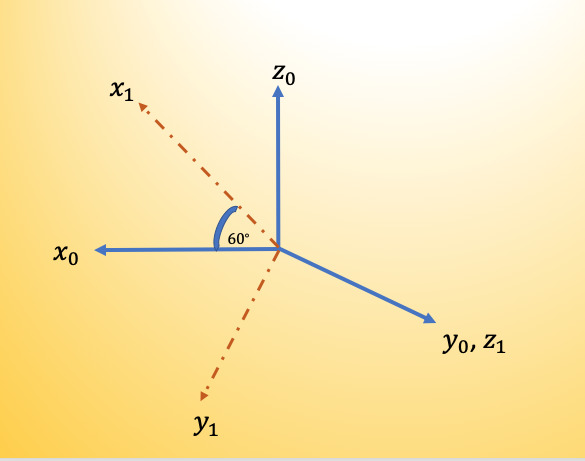
\includegraphics[width=\textwidth]{../Notes/figures/two_frames.jpg}
			\footnotesize{Relative orientation between two frames.}
		\end{column}
	\end{columns}
\end{frame}


\begin{frame}
	\frametitle{Local Parameterization of Rotations in SO(3)}
	\begin{theorem}[Euler]
		Any rotation in $SO(3)$ can be represented as a rotation about a fixed axis $\omega\in \reline^3$ through an angle $\theta \in [0, 2\pi)$.
	\end{theorem}
	\begin{columns}[]
		\begin{column}{.95\linewidth}
			\centering
			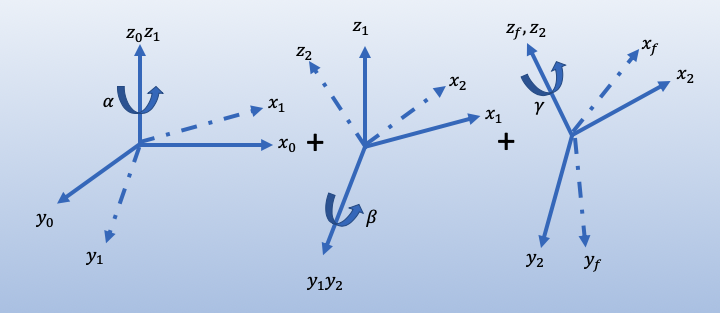
\includegraphics[width=\columnwidth]{../Notes/figures/zyz.png}
			\footnotesize{Relative orientation between two frames.}
		\end{column}
	\end{columns}
\end{frame}


\begin{frame}
	\frametitle{Local Parameterizations of SO(3)}
	\begin{block}{Rotation About Principal $\bm{x}$ Axis}
		\begin{align}
			\bm{R}_{\bm{x}}(\theta) = e^{\tilde{\bm{x}}\theta} 
			%
			= \begin{bmatrix}
				1 & 0 & 0 \\
				0 & \cos\theta & -\sin\theta \\
				%
				0 & \sin\theta & \cos\theta  
			\end{bmatrix}
		\end{align}
	\end{block}
	
	\begin{block}{Rotation About Principal $\bm{y}$ Axis}
		\begin{align}
			\bm{R}_{\bm{y}}(\phi) = e^{\tilde{\bm{y}}\phi} 
			%
			= \begin{bmatrix}
				-\cos\phi & 0 & -\sin\phi \\
				%
				0 & 1 & 0 \\
				-\sin \phi  & 0 & \cos \phi 
			\end{bmatrix}
		\end{align}
	\end{block}
\end{frame}


\begin{frame}
	\frametitle{Local Parameterizations of SO(3)}	
	\begin{block}{Rotation About Principal $\bm{z}$ Axis}
		\begin{align}
			\bm{R}_{\bm{z}}(\psi) = e^{\bm{\tilde{z}}\psi} 
			%
			= \begin{bmatrix}
				\cos\psi & -\sin\psi & 0\\
				%
				\sin \psi  & \cos \psi & 0 \\
				%
				0 & 0 & 1 
			\end{bmatrix}
		\end{align}
	\end{block}
\end{frame}

\begin{frame}
	\frametitle{Euler Angles as Parameterization of Rotations}
	``\textcolor{red}{\textit{Read Euler, read Euler, he is the master of us all}.}" -- Pierre-Simon Laplace.
	\begin{block}{Euler ($ZYZ$) Angles}
		\begin{align}
			\bm{R}_{ij}(\alpha, \beta, \gamma) &= \bm{R}_z(\alpha) \bm{R}_y(\beta) \bm{R}_z(\gamma) \\
			%
			& = \begin{bmatrix}
				c_\alpha & -s_\alpha & 0 \\
				%
				s_\alpha & c_\alpha & 0 \\
				%
				0 & 0 & 1
			\end{bmatrix}
			%
			\begin{bmatrix}
				c_\theta  & 0 & s_\theta\\
				%
				0  & 1 & 0 \\
				%
				-s_\theta  & 0 & c_\theta 
			\end{bmatrix} \nonumber \\
			%
			&= \begin{bmatrix}
				c_\alpha c_\beta c_\gamma - s_\alpha s_\gamma & -c_\alpha c_\beta s_\gamma - s_\alpha c_\gamma & c_\alpha s_\beta \\
				%
				s_\alpha c_\beta c_\gamma + c_\alpha s_\gamma & -s_\alpha c_\beta s_\gamma + c_\alpha c_\gamma  & s_\alpha s_\beta \\
				%
				-s_\beta c_\gamma & s_\beta s_\gamma & c_\beta
			\end{bmatrix} 
			\label{eq:zyz}
		\end{align} 
	\end{block}
\end{frame}

\begin{frame}
	\frametitle{Euler Angles as Parameterization of Rotations}
	``\textcolor{red}{\textit{The study of Euler's works will remain the best school for the different fields of mathematics, and nothing else can replace it}}." -- Carl Friedrich Gauss.
	\begin{block}{Euler ($ZYZ$) Angles. Case $\sin(\beta)>0$}
		Given an $R$ and $\sin(\beta)>0$, the Euler angles are:
		\begin{subequations}
			\begin{align}
				\beta &= \arctan 2(r_{33}, \sqrt{1 - r_{33}^2})  \label{eq:euler_a}\\
				\alpha &= \arctan 2(r_{23}/\sin \beta, r_{13}/\sin \beta) \label{eq:euler_b} \\
				\gamma &= \arctan 2 (r_{32}/\sin \beta, -r_{31}/\sin \beta)
			\end{align}
			\label{eq:euler}
		\end{subequations}
		%
		%\footnotesize{where $\arctan2(y, x)$ determines the quadrant of the angle based on the sign of $x$ and $y$}.
	\end{block}
\end{frame}

\begin{frame}
	\frametitle{Euler Angles as Parameterization of Rotations}
	\begin{block}{Euler ($ZYZ$) Angles. Case $\sin(\beta)<0$}
		Given an $R$ and $\sin(\beta)<0$, the Euler angles are:
		\begin{subequations}
			\begin{align}
				\beta &=  \arctan2(r_{33}, -\sqrt{1 - r_{33}^2})  \label{eq:euler_neg_a}\\
				\alpha &= \arctan 2(-r_{23}/\sin \beta, -r_{13}/\sin \beta) \label{eq:euler_neg_b} \\
				\gamma &= \arctan 2 (-r_{32}/\sin \beta, r_{31}/\sin \beta)
			\end{align}
			\label{eq:euler_neg}
		\end{subequations}
		%
		\footnotesize{\textcolor{red}{Euler angles are not unique} owing to the sign of the angle about which the $y$ axis rotates!}
	\end{block}
\end{frame}

\begin{frame}
	\frametitle{Euler Angles Drawbacks}
	\begin{block}{Drawbacks}
		\begin{description}
			\item Lack of \textcolor{red}{smooth, global solutions} to Euler angles from rotation;
			\item \textcolor{purple}{Singularities} at $\rot = \identity$;
			\item \textcolor{magenta}{Possible infinite representation of Euler angles at specific configurations} e.g. $\rot(\theta, 0, -\theta)=\identity$.
		\end{description}
	\end{block}
\end{frame}


\begin{frame}
	\frametitle{Yaw, Pitch, and Roll Axes}
	\begin{columns}[]
		\begin{column}{.45\linewidth}
			\begin{block}{Fick angles}
				Otherwise called the \textcolor{magenta}{yaw, pitch, and roll angles}. $\bm{R}_{ij}$ found by \textcolor{gray}{rotating about the $x-$axis}  (roll), then  a \textcolor{cyan}{rotation about the $y-$axis (pitch)}, and finally a rotation about \textcolor{brown}{$z-$axis} -- all in the body frame. 
			\end{block}
		\end{column}
		\begin{column}{.55\linewidth}
			\centering
			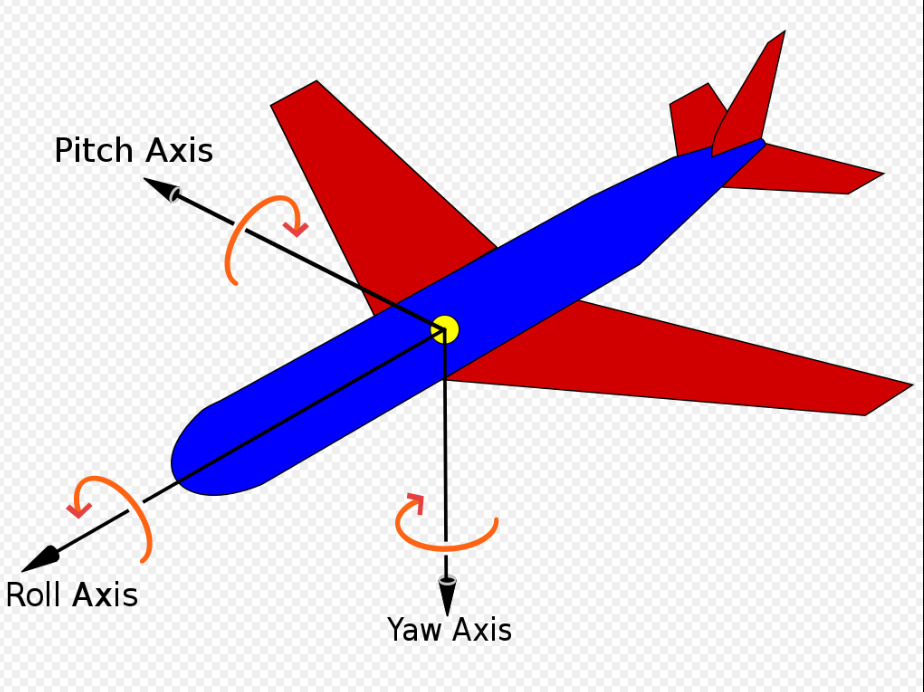
\includegraphics[width=\textwidth]{figures/yawpitchroll.jpg}
			\footnotesize{Aircraft Principal Axes in the right-hand frame. Courtesy of Wikimedia commons.}
		\end{column}
	\end{columns}
\end{frame}


\begin{frame}
	\frametitle{Quaternions}
	\begin{block}{Global Parameterization of Rotations}
		  Instead of \textcolor{magenta}{locally parameterizing the $SO(3)$ group}, \textcolor{blue}{quaternions}, unlike rotation matrices, \textcolor{brown}{globally parameterize the \textit{SO(3)} Lie Group}.
	\end{block}
	
	\begin{block}{Quaternions}
		Formally, we represent a \textcolor{blue}{quaternion} as follows:
		%
		\begin{align}
			Q = q_0 + q_x \bm{i} + q_y \bm{j} + q_z \bm{k},
		\end{align}
		%
		where $q_0 \in \bb{R}$ is the scalar component of $Q$ and $\bm{q} = (q_x, q_y, q_z) \in \bb{R}^3$ is the vector component.
	\end{block}
\end{frame}

\begin{frame}
	\frametitle{Quaternions}
	\begin{block}{Quaternions}
		%
		The \textcolor{magenta}{unit quaternions} are the \textcolor{cyan}{subset of all $Q \in \bb{Q}$ such that $\|Q\| = 1$}. For a rotation matrix $R = \text{exp}(\hat{\omega}\theta)$, we have the unit \textcolor{blue}{quaternion} as 
		%
		\begin{align}
			Q = \left(\cos(\theta/2), \omega \sin \left(\theta/2\right) \right),
		\end{align}
		%
		where $\omega \in \bb{R}^3$ is the \textcolor{brown}{axis of orientation} and $\theta \in \bb{R}$ is the \textcolor{brown}{angle of rotation}.
	\end{block}
\end{frame}

\begin{frame}
	\frametitle{Other Parameterization of Rotations}
	\begin{block}{Fick ($ZYX$), Helmholtz ($YZX$) Angles.}
		 We could \textcolor{red}{permute the order of rotation} such as rotating successively about \textcolor{cyan}{different axes}. Examples include \textcolor{blue}{successive rotations about $ZYX$ axes for the Fick angles} and \textcolor{brown}{successive rotations about $YZX$ axes for Helmholtz angles}.
	\end{block}
	
	\begin{block}{Fick ($ZYX$) and Helmholtz ($YZX$) Angles.}
		These avoid \textcolor{blue}{Euler angle} \textcolor{red}{singularities} at $\bm{R} = \bm{I}$. This does not preclude \textcolor{red}{singularities at other configurations}.
	\end{block}
\end{frame}


\begin{frame}
	\frametitle{Summary of Parameterization of Rotations}
	\begin{tcolorbox}[title=Summary of Parameterizations]
		Rotation matrices can be parameterized in one of many ways depending on our use case. The common examples of parameterizations are 
		%
		\begin{inparaenum}[\itshape (1)\upshape] \newline
			\item Axis-Angle representation; \newline
			\item Euler  angles ($ZYZ$) representation; \newline
			\item Fick  angles (\ie $ZYX$ or yaw, pitch and roll)  representation; \newline
			\item Helmholtz angles (or $YZX$) angles representation; and \newline
			\item Quaternions.
		\end{inparaenum}
		
	\end{tcolorbox}
\end{frame}